\chapter{Arquitectura IVOA}

El \gls{vo} es un framework que ayuda a resolver distintos problemas que enfrenta la comunidad astronómica internacional. Uno de los problemas está relacionado al acceso a los datos, por lo que en IVOA diseñaron tecnologías y estándares formalmente definidos, que permitan el acceso unificado y transparente a distintos servidores con datos astronómicos.

El beneficio que conlleva es considerable, ya que estos estándares, protocolos, tecnologías y arquitectura, ayudan a la comunidad al proceso de creación de servicios, portales web, aplicaciones de escritorio, etc. Todo visto del punto de vista de ingeniería de software.

\section{Arquitectura VO por nivel}

\gls{ivoa} dentro de sus documentos presenta distintos niveles de arquitectura \cite{ivoaArq}, con el objetivo de ir aclarando incrementalmente las funcionalidades (basadas en necesidades) que requiere un VO.

\subsection{Arquitectura Nivel 0}

La arquitectura más básica que aclara el concepto de VO, se compone de 3 capas (Img.~\ref{img:arq0}):

\begin{figure}[ht!]
	\centering
	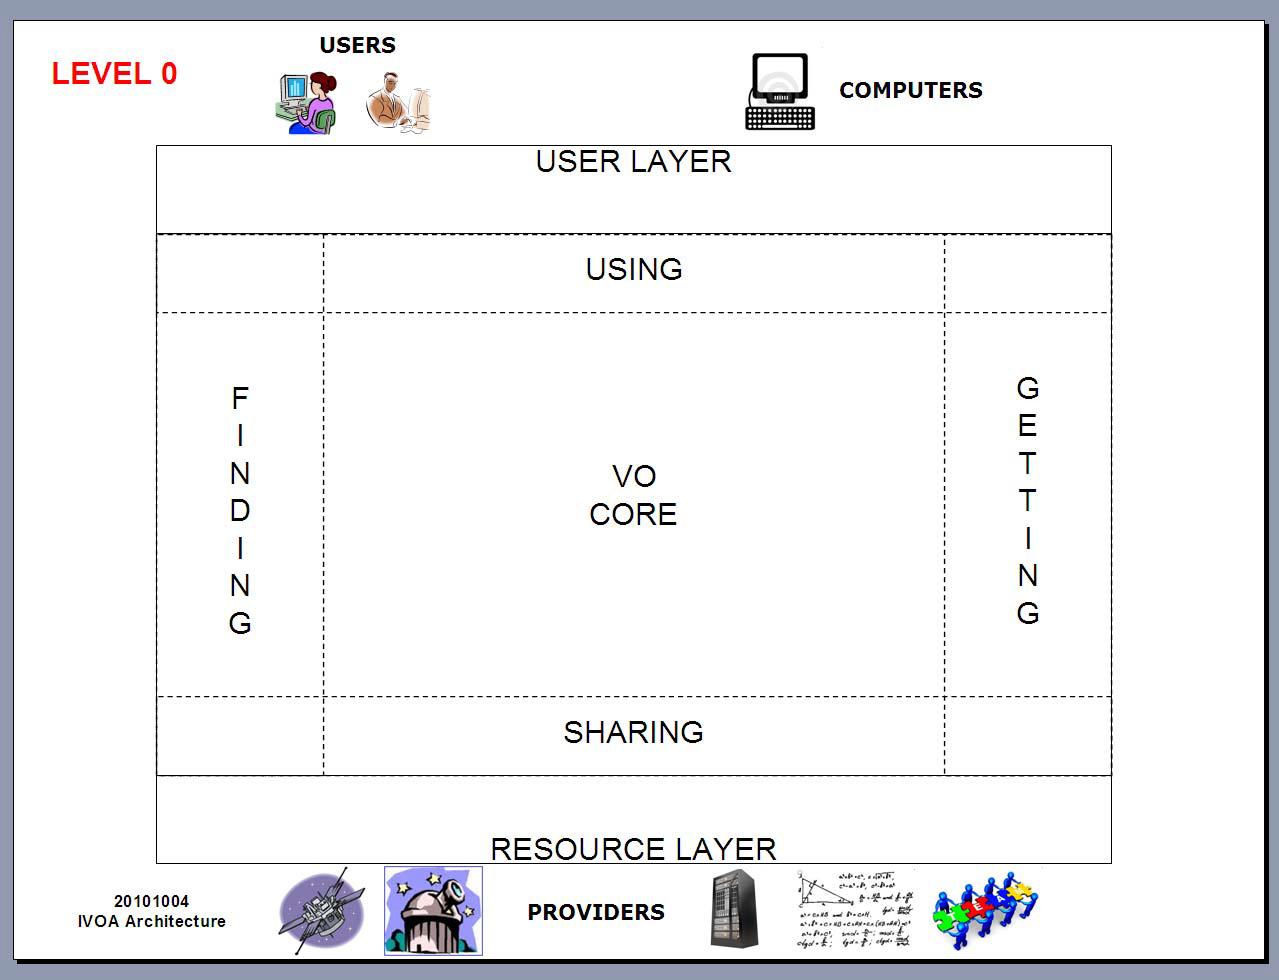
\includegraphics[scale=.2]{arq0}
	\caption{Arquitectura nivel 0.}
	\label{img:arq0}
\end{figure}

\begin{enumerate}
	\item Capa de recursos: compilado de datos astronómicos provenientes de distintos instrumentos.
	\item Capa de usuarios: investigadores que buscan consumir datos.
	\item Capa intermedia: es la capa que permite conectar las dos capas anteriores de manera transparente para los investigadores. Esta interacción se puede llevar a cabo buscando u obteniendo datos.
\end{enumerate}

\subsection{Arquitectura Nivel 1}

La arquitectura nivel 1 mantiene la misma cantidad de capas pero se especifica aún más (Img.~\ref{img:arq1}):

\begin{figure}[ht!]
	\centering
	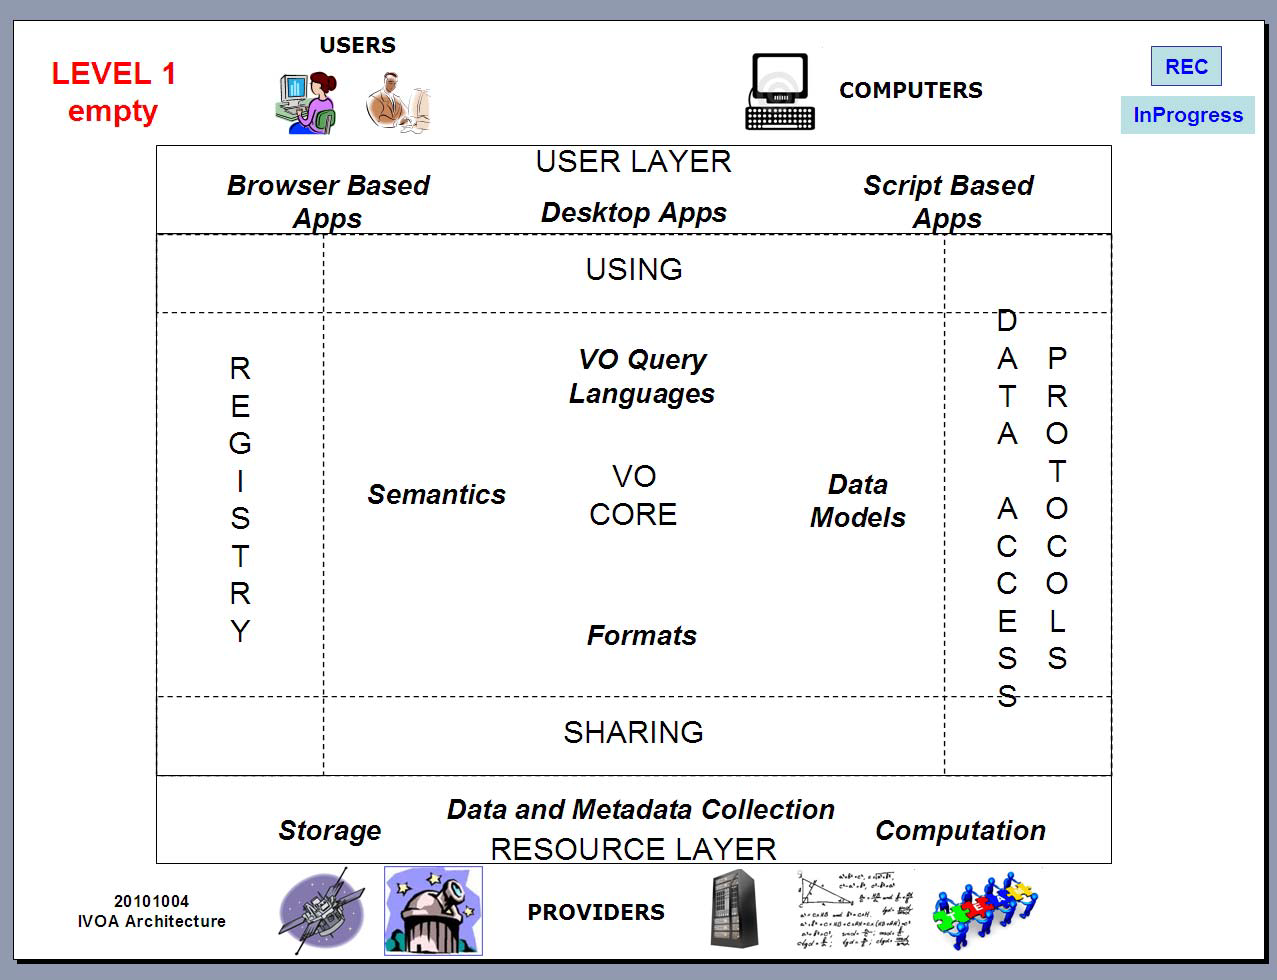
\includegraphics[scale=.2]{arq1}
	\caption{Arquitectura nivel 1.}
	\label{img:arq1}

\end{figure}

\begin{enumerate}
	\item Capa de recursos: está compuesto de una colección de datos y provenientes de distintos servidores.
	\item Capa de usuarios: un consumidor puede querer acceder a los datos desde un navegador, escritorio, o mediante un script.
	\item Capa intermedia: crea un framework para compartir los datos, compuesto por \gls{voql}, \emph{Data Models}, \emph{semantics}, \emph{Formats}.
\end{enumerate}

\subsection{
Arquitectura Nivel 2}

La arquitectura nivel 2 es lo que se entiende por un VO regido por estándares y protocolos de IVOA. La idea de esta figura es seccionar cada estándar relacionándolo específicamente a la capa a la cual pertenece (Img.~\ref{img:arq2}).


\begin{figure}[ht!]
	\centering
	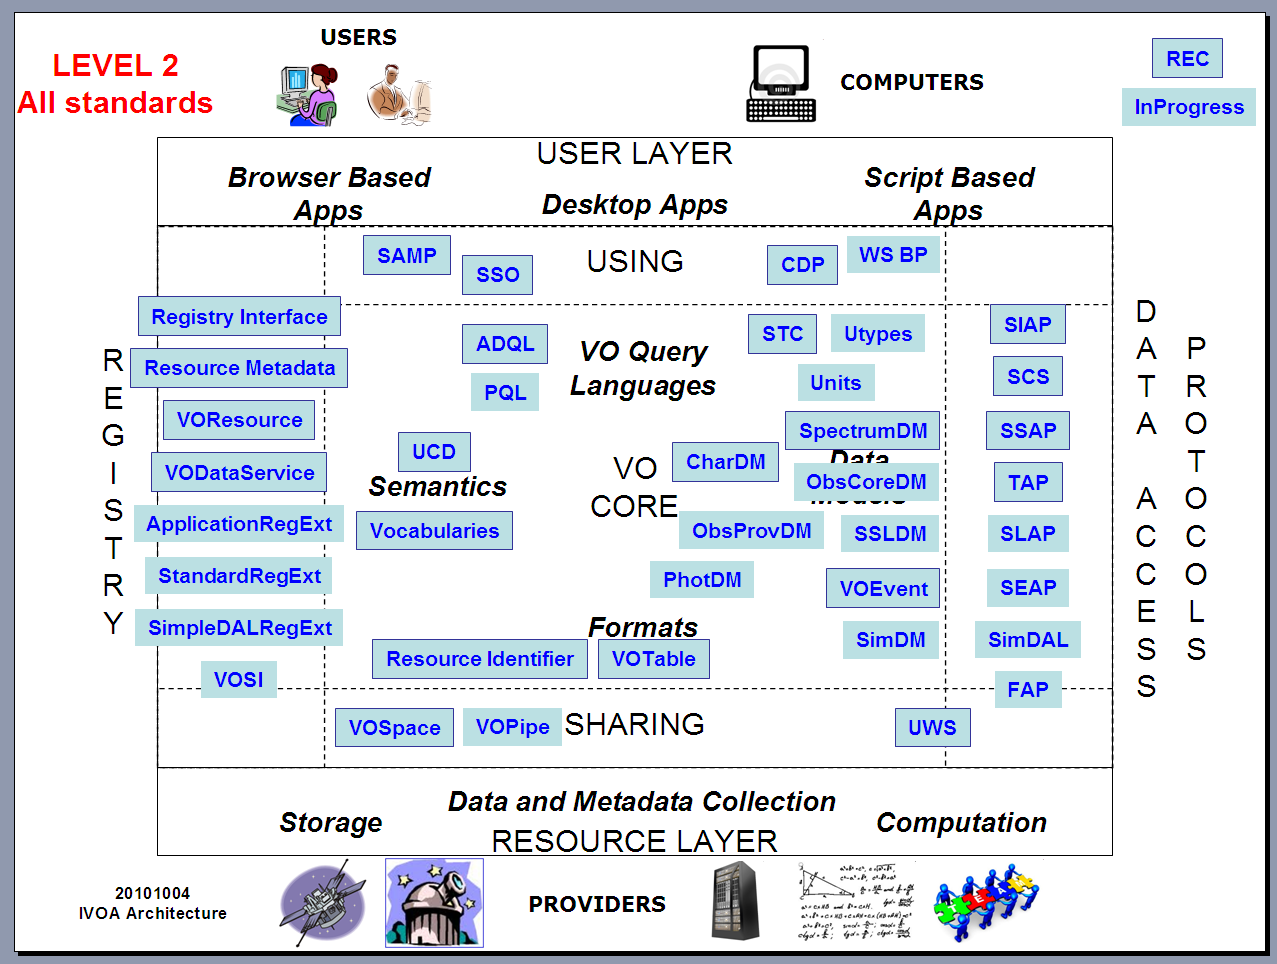
\includegraphics[scale=.2]{arq2}
	\caption{Arquitectura nivel 2.}
	\label{img:arq2}
\end{figure}
